\documentclass[]{article}
\usepackage{lmodern}
\usepackage{amssymb,amsmath}
\usepackage{ifxetex,ifluatex}
\usepackage{fixltx2e} % provides \textsubscript
\ifnum 0\ifxetex 1\fi\ifluatex 1\fi=0 % if pdftex
  \usepackage[T1]{fontenc}
  \usepackage[utf8]{inputenc}
\else % if luatex or xelatex
  \ifxetex
    \usepackage{mathspec}
  \else
    \usepackage{fontspec}
  \fi
  \defaultfontfeatures{Ligatures=TeX,Scale=MatchLowercase}
\fi
% use upquote if available, for straight quotes in verbatim environments
\IfFileExists{upquote.sty}{\usepackage{upquote}}{}
% use microtype if available
\IfFileExists{microtype.sty}{%
\usepackage{microtype}
\UseMicrotypeSet[protrusion]{basicmath} % disable protrusion for tt fonts
}{}
\usepackage[margin=1in]{geometry}
\usepackage{hyperref}
\hypersetup{unicode=true,
            pdftitle={Whale's Tale Staffing Analysis With Depts},
            pdfauthor={Allocate Analytics},
            pdfborder={0 0 0},
            breaklinks=true}
\urlstyle{same}  % don't use monospace font for urls
\usepackage{longtable,booktabs}
\usepackage{graphicx,grffile}
\makeatletter
\def\maxwidth{\ifdim\Gin@nat@width>\linewidth\linewidth\else\Gin@nat@width\fi}
\def\maxheight{\ifdim\Gin@nat@height>\textheight\textheight\else\Gin@nat@height\fi}
\makeatother
% Scale images if necessary, so that they will not overflow the page
% margins by default, and it is still possible to overwrite the defaults
% using explicit options in \includegraphics[width, height, ...]{}
\setkeys{Gin}{width=\maxwidth,height=\maxheight,keepaspectratio}
\IfFileExists{parskip.sty}{%
\usepackage{parskip}
}{% else
\setlength{\parindent}{0pt}
\setlength{\parskip}{6pt plus 2pt minus 1pt}
}
\setlength{\emergencystretch}{3em}  % prevent overfull lines
\providecommand{\tightlist}{%
  \setlength{\itemsep}{0pt}\setlength{\parskip}{0pt}}
\setcounter{secnumdepth}{0}
% Redefines (sub)paragraphs to behave more like sections
\ifx\paragraph\undefined\else
\let\oldparagraph\paragraph
\renewcommand{\paragraph}[1]{\oldparagraph{#1}\mbox{}}
\fi
\ifx\subparagraph\undefined\else
\let\oldsubparagraph\subparagraph
\renewcommand{\subparagraph}[1]{\oldsubparagraph{#1}\mbox{}}
\fi

%%% Use protect on footnotes to avoid problems with footnotes in titles
\let\rmarkdownfootnote\footnote%
\def\footnote{\protect\rmarkdownfootnote}

%%% Change title format to be more compact
\usepackage{titling}

% Create subtitle command for use in maketitle
\newcommand{\subtitle}[1]{
  \posttitle{
    \begin{center}\large#1\end{center}
    }
}

\setlength{\droptitle}{-2em}

  \title{Whale's Tale Staffing Analysis With Depts}
    \pretitle{\vspace{\droptitle}\centering\huge}
  \posttitle{\par}
    \author{Allocate Analytics}
    \preauthor{\centering\large\emph}
  \postauthor{\par}
      \predate{\centering\large\emph}
  \postdate{\par}
    \date{April 10, 2018}


\begin{document}
\maketitle

\paragraph{Question To Answer: How can sales data help inform staffing
levels through the day through each month of the
year?}\label{question-to-answer-how-can-sales-data-help-inform-staffing-levels-through-the-day-through-each-month-of-the-year}

\paragraph{Approach To Answer
Question:}\label{approach-to-answer-question}

\begin{enumerate}
\def\labelenumi{\arabic{enumi}.}
\item
  Visualize 2017 sales by hour for each day of the year in order to see
  trends (also visualize 2016 to confirm it's fairly similar to 2017)
\item
  Group together similar days into a number of ``sales profiles'' for
  consistency and simplicity.
\item
  Plot the range of sales that happen through the day for each of the 10
  profiles.
\end{enumerate}

\subsection{Sales By Hour For Each Day of
2017}\label{sales-by-hour-for-each-day-of-2017}

\includegraphics{prelim.staffing_files/figure-latex/calendar.17.plot-1.pdf}

\subsection{Comments and Trends}\label{comments-and-trends}

1 Almost no big days until 2nd weekend of April and then it's Fri, Sat,
Sun

2 Weekdays start getting consistently big after Memorial Day

3 Weekdays slow down after Labor Day

4 October weekdays even slower than September

5 Beginning around Halloween Saturday is really the main big weekend day
until the week before Xmas and except for Thanksgiving weekend

\subsection{Sales By Hour For Each Day of
2016}\label{sales-by-hour-for-each-day-of-2016}

\includegraphics{prelim.staffing_files/figure-latex/calendar.16.plot-1.pdf}

\subsection{Profiles of Sales For
Staffing}\label{profiles-of-sales-for-staffing}

\begin{figure}
\centering
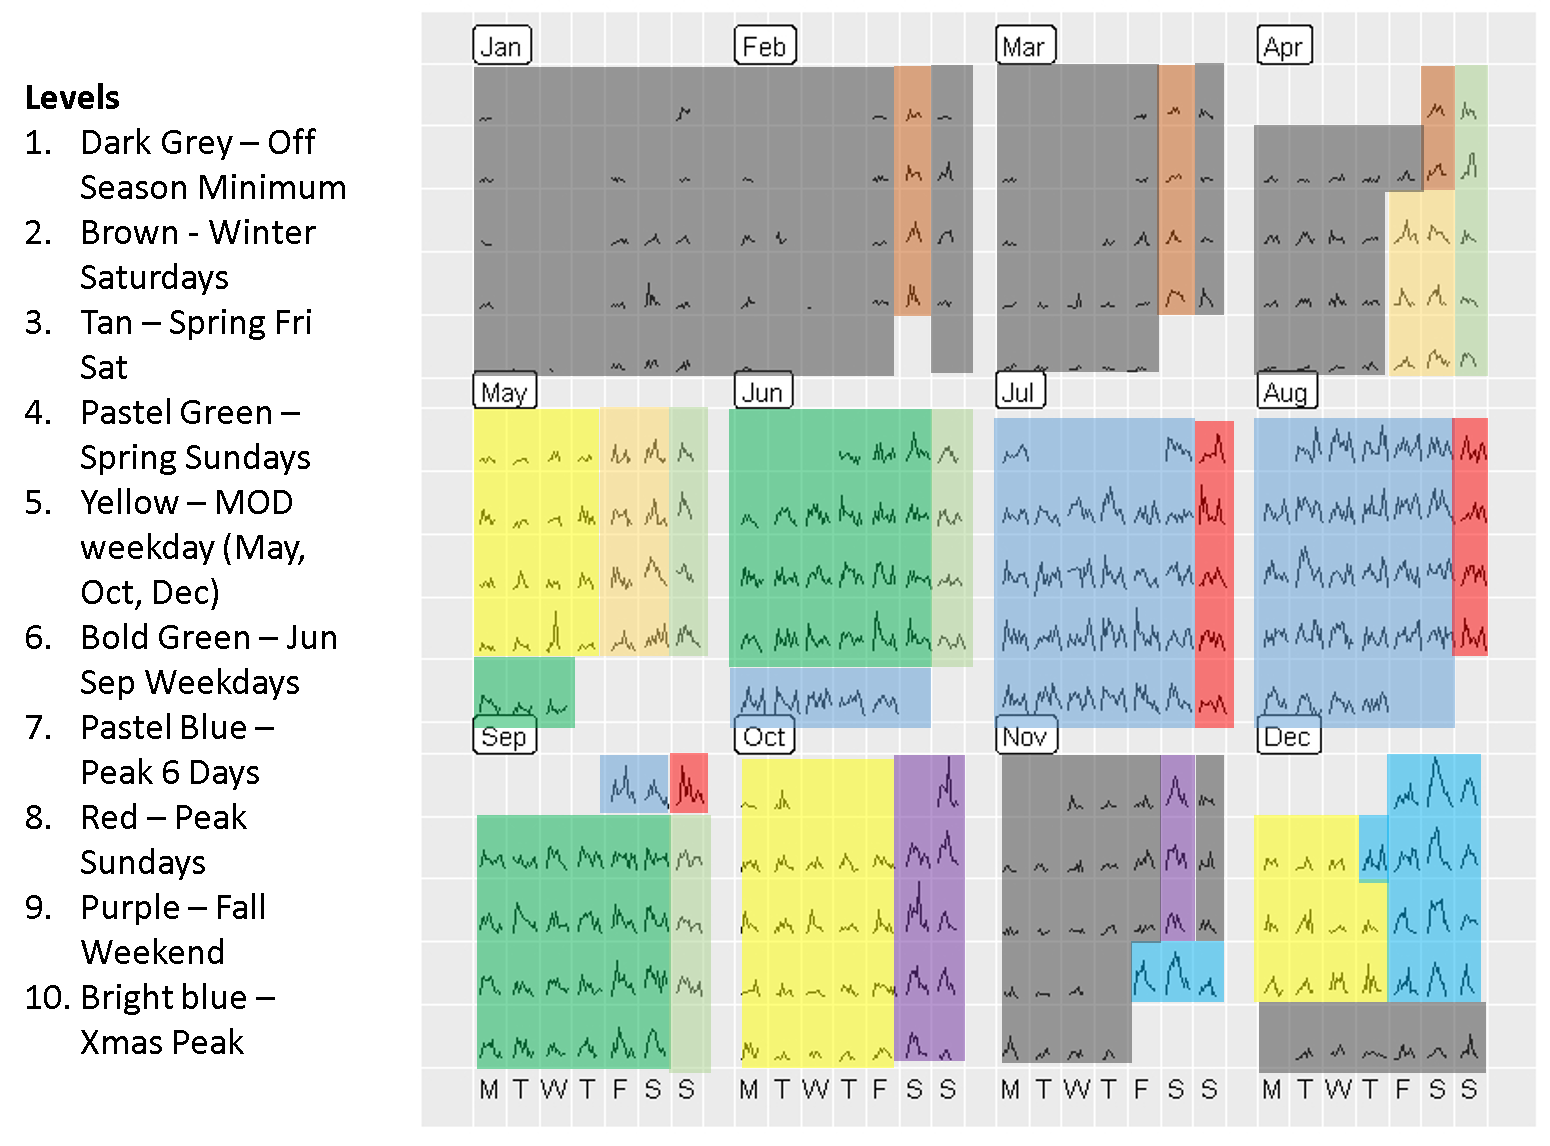
\includegraphics{day.sorting.staffing.png}
\caption{``Days of 2017 sorted into 10 profiles for staffing''}
\end{figure}

\newpage

\section{Sales Ranges of Profiles}\label{sales-ranges-of-profiles}

The next 10 plots show the range of sales that have occurred for each
hour of the day. The darkest, largest blue range represents where sales
occur that hour 95\% of the time. The next slightly lighter blue range
represents where hourly sales will fall 75\%. The smallest, lightest
blue contains hourly sales 50\% of the time. The red ribbon is the
average sales level for that hour.

My initial recommendation is to aim for the top of the 50\% range (the
lightest blue range, corresponding to about \$400 for 12 noon for the
first profile). Since the store being fully staffed as 6 people and the
minimum is 2, that informs the staffing levels. The highest the 50\%
range gets in mid-July is about \$1200/hr and the lowest is roughly
\$400/hr. This translates to the table below:

\subparagraph{Approximate Staffing Needs At Hourly Sales
Levels}\label{approximate-staffing-needs-at-hourly-sales-levels}

\begin{longtable}[]{@{}lr@{}}
\toprule
Sales.Per.Hour & Staff.Needed\tabularnewline
\midrule
\endhead
\$400 & 2\tabularnewline
\$600 & 3\tabularnewline
\$800 & 4\tabularnewline
\$1000 & 5\tabularnewline
\$1200 & 6\tabularnewline
\bottomrule
\end{longtable}

Below are the plots of each profile:

\newpage

\subsection{\#1 Off Peak Minimum Staffing - Dark
Grey}\label{off-peak-minimum-staffing---dark-grey}

This first one represents all the very low sales days, and the demands
of customers and sales are unlikely to require more than 2 staff at any
one time.

\includegraphics{prelim.staffing_files/figure-latex/Off.Peak.Min-1.pdf}

\subsubsection{Departments for \#1 Off Peak Minimum
Staffing}\label{departments-for-1-off-peak-minimum-staffing}

\includegraphics{prelim.staffing_files/figure-latex/unnamed-chunk-1-1.pdf}

\subsection{\#2 Winter Saturdays - Brown - Feb, Mar, early
April}\label{winter-saturdays---brown---feb-mar-early-april}

\includegraphics{prelim.staffing_files/figure-latex/Winter.Saturdays-1.pdf}

\subsubsection{Departments for \#2 Winter
Saturdays}\label{departments-for-2-winter-saturdays}

\includegraphics{prelim.staffing_files/figure-latex/unnamed-chunk-2-1.pdf}

\subsection{\#3 Spring Fri-Sat - Tan - Mid-April to
May}\label{spring-fri-sat---tan---mid-april-to-may}

\includegraphics{prelim.staffing_files/figure-latex/Spring.Fri.Sat.Tan.Mid.ApriltoMay-1.pdf}

\subsubsection{Departments for \#3 Spring
Fri-Sat}\label{departments-for-3-spring-fri-sat}

\includegraphics{prelim.staffing_files/figure-latex/unnamed-chunk-3-1.pdf}

\subsection{\#4 Spring Sundays - Pastel Green - April-June
Sundays}\label{spring-sundays---pastel-green---april-june-sundays}

\includegraphics{prelim.staffing_files/figure-latex/Spring.Sundays-1.pdf}

\subsubsection{Departments for \#4 Spring
Sundays}\label{departments-for-4-spring-sundays}

\includegraphics{prelim.staffing_files/figure-latex/unnamed-chunk-4-1.pdf}

\subsection{\#5 May, Oct, Dec Weekdays -
Yellow}\label{may-oct-dec-weekdays---yellow}

\includegraphics{prelim.staffing_files/figure-latex/May.Oct.Dec.Weekdays-1.pdf}

\subsubsection{Departments for \#5 May, Oct, Dec
Weekdays}\label{departments-for-5-may-oct-dec-weekdays}

\includegraphics{prelim.staffing_files/figure-latex/unnamed-chunk-5-1.pdf}

\subsection{\#6 Jun/Sep 6 Days - Bold
Green}\label{junsep-6-days---bold-green}

\includegraphics{prelim.staffing_files/figure-latex/Jun.Sep.6.days-1.pdf}

\subsubsection{Departments for \#6 Jun/Sep 6
Days}\label{departments-for-6-junsep-6-days}

\includegraphics{prelim.staffing_files/figure-latex/unnamed-chunk-6-1.pdf}

\subsection{\#7 Peak 6 Days - Pastel Blue - Mon-Sat Jul \&
Aug}\label{peak-6-days---pastel-blue---mon-sat-jul-aug}

\includegraphics{prelim.staffing_files/figure-latex/peak.6.days-1.pdf}

\subsubsection{Departments for \#7 Peak 6
Days}\label{departments-for-7-peak-6-days}

\includegraphics{prelim.staffing_files/figure-latex/unnamed-chunk-7-1.pdf}

\subsection{\#8 Peak Sundays - Red - July-Labor Day
Sundays}\label{peak-sundays---red---july-labor-day-sundays}

\includegraphics{prelim.staffing_files/figure-latex/Peak.Sundays-1.pdf}

\subsubsection{Departments for \#8 Peak
Sundays}\label{departments-for-8-peak-sundays}

\includegraphics{prelim.staffing_files/figure-latex/unnamed-chunk-8-1.pdf}

\subsection{\#9 Fall Weekend - Purple - Oct Sat/Sun \& Nov
Sat}\label{fall-weekend---purple---oct-satsun-nov-sat}

\includegraphics{prelim.staffing_files/figure-latex/Fall.Weekend-1.pdf}

\subsubsection{Departments for \#9 Fall
Weekend}\label{departments-for-9-fall-weekend}

\includegraphics{prelim.staffing_files/figure-latex/unnamed-chunk-9-1.pdf}

\subsection{\#10 Xmas Peak - Bright Blue - Fri, Sat, Sun
Dec}\label{xmas-peak---bright-blue---fri-sat-sun-dec}

\includegraphics{prelim.staffing_files/figure-latex/Xmas.Peak-1.pdf}

\subsubsection{Departments for \#10 Xmas
Peak}\label{departments-for-10-xmas-peak}

\includegraphics{prelim.staffing_files/figure-latex/unnamed-chunk-10-1.pdf}


\end{document}
